\documentclass[12pt]{article}
\usepackage[a4paper]{geometry}
\usepackage[utf8]{inputenc}
\usepackage[nottoc]{tocbibind}
\usepackage{fancyhdr}
\usepackage{lastpage}
\usepackage{graphicx, wrapfig, subcaption, setspace, booktabs}
\usepackage{graphicx}
\usepackage{hyperref}
\usepackage[T1]{fontenc}
\usepackage[font=small, labelfont=bf]{caption}
\usepackage{multirow}
\usepackage[protrusion=true, expansion=true]{microtype}
\usepackage[spanish]{babel}
\usepackage{sectsty}
\usepackage{url, lipsum}
\usepackage[T1]{fontenc}
\usepackage{icomma}
\usepackage{siunitx}
\usepackage{gensymb}
\usepackage{ragged2e}
\usepackage{amsmath}
\usepackage{comment}
\usepackage{enumerate}
\usepackage{anysize}
\usepackage{biblatex}
\addbibresource{bibliography.bib}


\newcommand{\HRule}[1]{\rule{\linewidth}{#1}}
\onehalfspacing
\setcounter{tocdepth}{5}
\setcounter{secnumdepth}{5}

\begin{document}

\begin{titlepage}

\title{\normalsize 
        \begin{center}
        
\includegraphics[height=6cm]{LogoUnison.jpg}
        \end{center}
        \LARGE \textsc{\textbf{Universidad De Sonora}} \\ \bigskip
		\Large División de Ciencias Exactas y Naturales \\
        Licenciatura en Física \\ \bigskip
        \bigskip
        T E S I S
		\\ [0.1cm]  
		\HRule{2pt} \\
		\Large \textbf{{Studying Dark Matter \& Dark Energy}} \\
		\HRule{2pt} \\
		\normalsize \vspace*{0.001\baselineskip}}
        
\date{\bigskip \Large Hermosillo, Sonora  \hspace*{\fill} Octubre de 2020}

        
\author{
		\Large\textbf{Luis Fernando Duarte Gonzalí} \\ \bigskip
        \\ \bigskip}
       \end{titlepage}
       \maketitle
       



\newpage
\tableofcontents
\newpage
\pagestyle{plain}
\section{Introducción}
\noindent A lo largo de la historia el ser humano siempre se ha preguntado por la estructura de las cosas, o cuál es la parte más pequeña de la materia que nos rodea y esa misma cuestión ha escalado a tal punto de preguntarnos de qué está compuesto nuestro universo en su totalidad. En la actualidad nos hemos encontrado con que la materia que percibimos a simple vista y medimos en los laboratorios forma la mínima parte de la composición del vasto universo.

\subsection{Componentes del Universo}

Materia oscura (DM) y energía oscura (DE), ambas son consideradas piezas esenciales perdidas del rompecabezas cósmico. Existe una gran cantidad de evidencias que apoyan a la existencia de materia oscura y energía oscura en nuestro universo basado en observaciones astronómicas. En el modelo cosmológico actual es bien conocido que la distribución de densidad de energía de las tres componentes del universo son aproximadamente; 68\% energía oscura, 27\% materia oscura y 5\% materia bariónica. Menos del 1\% lo conforma la radiación (fotones y neutrinos).

\subsubsection{Materia Oscura}
\noindent La naturaleza misma de la materia oscura sigue siendo una incógnita y un problema a resolver en la física moderna. Nos ha llevado a modificar la propia teoría de la relatividad (GR) y proponer modelos en los que la parte mínima de la materia oscura radica en una teoría más allá del modelo estándar (SM). Estamos hablando de un conflicto que envuelve a la investigación en la intersección entre la astrofísica, la cosmología y la física de partículas.

Le llamamos materia oscura a aquella materia que no interacciona, o por lo menos no tan fuerte como la materia ordinaria (bariónica), con los campos electromagnéticos, fuerte y débil. La manera más común y con la que se ha detectado este tipo de materia es por medio de la interacción gravitacional. \cite{Faber_2006}

En realidad, la necesidad de introducir el concepto de materia oscura fue propuesto inicialmente por Zwicky (1933) quien se percató de que la velocidad rotacional de las galaxias individuales que se encuentran en el clúster de Coma eran muy grandes y que la única forma en que el clúster estuviera ligado gravitacionalmente es que la suma de sus partes (galaxias) fuera mucho menor que la masa total.

Al momento de realizar observaciones astronómicas de una galaxia se toman datos hasta el punto en que no se logren detectar más componentes luminosas galácticas (estrellas y/o gas). 

Con la tercera ley de Kepler podemos determinar la forma de las curvas de rotación galaxias individuales midiendo la distancia de la componente luminosa al núcleo y su velocidad en ese punto. \cite{Sahni_2004}

\begin{equation}
    v(r) = \sqrt{\frac{GM(r)}{r}}
\end{equation}
 Lo que se detecta en una gran cantidad de observaciones es que la velocidad no decae como se espera $v(r) \propto r^{-\frac{1}{2}}$. De hecho se observa que la velocidad se mantiene constante y en algunos casos puede llegar a aumentar. Entonces la masa se convierte en un factor dependiente de la distancia radial. Esto nos sugiere que aun sin tener esas componentes luminosas de las galaxias, su masa sigue creciendo conforme nos alejamos del centro de ellas por lo que podemos establecer la presencia de materia oscura. Ver las figuras \ref{rotationbegeman} y \ref{rotationvera}. 
\begin{figure}
    \centering
    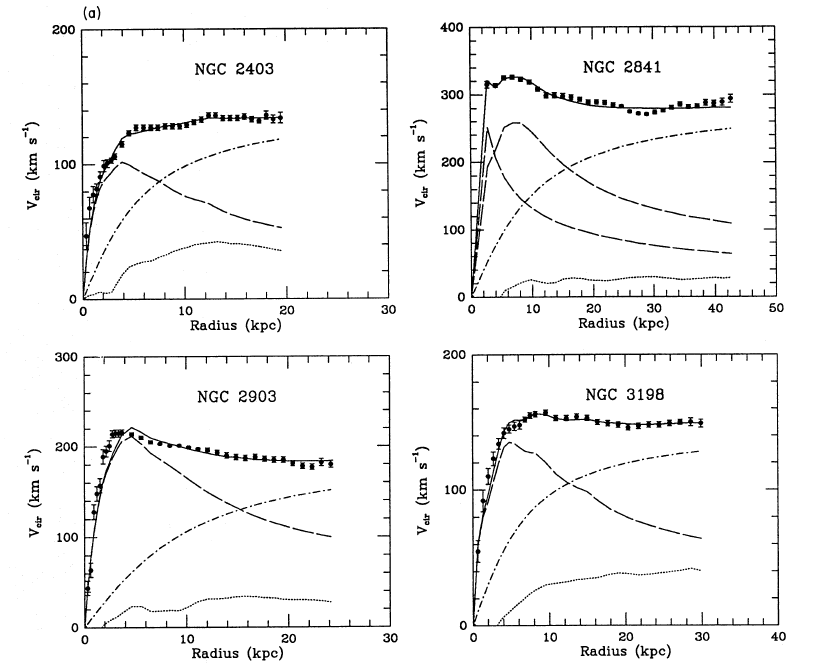
\includegraphics[scale=0.35]{Figures/galaxyrotationcurves.png}
    \caption{Curvas de rotación de algunas galaxias de espiral, con contribución de componentes luminosos (rayas), gas (puntos) y halo de materia oscura (puntos y rayas). Los bloques cuadrados son datos de la observación. La linea sólida es el ajuste del modelo de materia oscura. Begeman et al. (1991)}
    \label{rotationbegeman}
\end{figure}
\begin{figure}[htb]
    \centering
    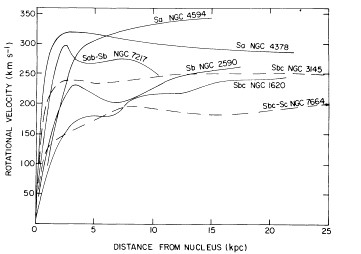
\includegraphics[scale=.6]{Figures/galaxyrotationvera.jpg}
    \caption{Curvas de rotación de algunas galaxias espiral. Por Rubin et al. (1978)}
    \label{rotationvera}
\end{figure}
\\

Hasta ahora se ha establecido con cierto grado de confianza que la constituyente o constituyentes de los componentes de la materia oscura no pueden ser cualquier tipo de materia ordinaria (bariónica). Lo que nos ha llevado a proponer candidatos a materia oscura fuera del modelo estándar de partículas actual. (Sección 1.2)

\subsubsection{Energía Oscura}
\noindent Una de las pruebas que tenemos de que el Big Bang ha ocurrido, es que podemos observar la huella que ha dejado apuntando los radiotelescopios al cielo a cualquier hora del día. Estamos hablando del fondo cósmico de microondas (CMB).

Otra de las pruebas de que el universo tuvo un inicio es que está en expansión y no solo se expande, sino que lo hace a un ritmo acelerado. De hecho se da la expansión del universo por la composición de la energía y masa dentro del mismo. Por lo tanto la materia ordinaria aporta cierta parte para que se dé la expansión aunque sea en menor parte. De hecho la mayor contribuyente sería a lo que le llamamos Energía Oscura.

Uno de los candidatos más conocidos para energía oscura es aquella representada en las ecuaciones de Einstein como el término de la energía del vacío. De hecho los datos existentes se adecúan bien al comportamiento estacionario y sin perturbaciones espacialmente de la densidad de la energía del vacío. Aunque por otro lado existen muchos otros modelos propuestos para le energía oscura como la teoría de la relatividad general modificada, campos nuevos y algunos más. Activando un área de la cosmología moderna en donde se trata de investigar y describir la expansión del universo con ciertos modelos y simulaciones buscando explicación para el ritmo de aceleración y densidad de fluctuaciones.

Está claro que uno de los problemas es saber cómo identificar propiedades de esta componente del universo

\href{Sahni_2004}{hola}

\subsubsection{Materia Bariónica}

\subsection{Candidatos a Materia Oscura}
\subsubsection{Weakly Interacting Massive Particles (WIMPs)}
\subsubsection{Axions and Strong CP Problem}
\subsubsection{Neutrinos as DM}

\subsection{Métodos de Medición}
\subsubsection{Gravitational Lensing}
\subsubsection{Baryon Acoustic Oscillations}

\printbibliography


\end{document}
